\documentclass[12pt,a4paper]{ctexart}

\usepackage{amsmath,amssymb,bm,booktabs,caption,enumitem,fancyhdr,float,geometry,graphicx,hyperref,tcolorbox}

\geometry{left=25mm,right=25mm,top=25mm,bottom=25mm}
\graphicspath{{assets/figures/}}
\hypersetup{colorlinks=true,linkcolor=blue,citecolor=blue,urlcolor=blue}
\setlength{\parindent}{2em}
\setlength{\parskip}{0.35em}
\setlength{\headheight}{15pt}
\pagestyle{fancy}
\fancyhf{}
\lhead{Material-Volume EP Flux}
\rhead{\thepage}

\newcommand{\p}{\partial}
\newcommand{\dd}{\,\mathrm d}
\newcommand{\D}{\mathrm D}
\newcommand{\meanV}[1]{\left\langle #1\right\rangle_V}
\newcommand{\fluc}[1]{#1^{\dagger}}
\newcommand{\bx}{\boldsymbol x}
\newcommand{\bu}{\boldsymbol u}
\newcommand{\bU}{\boldsymbol U}
\newcommand{\bR}{\boldsymbol R}
\newcommand{\bV}{\boldsymbol V}
\newcommand{\bt}{\boldsymbol t}
\newcommand{\bn}{\boldsymbol n}
\newcommand{\PP}{\boldsymbol{\mathsf P}_{\perp}}
\newcommand{\GG}{\mathcal G}
\newcommand{\TT}{\mathcal T}
\newcommand{\VV}{\mathcal V_c}
\newcommand{\SSS}{\partial\mathcal V_c}

\title{\bfseries 大曲率下的 Material-Volume EP Flux：\\从细涡管坐标到三维 coherent 材料体}
\author{ZONCA-EP-FLUX-TEST}
\date{2026 年 9 月 1 日}

\begin{document}
\maketitle

本文档接在 \texttt{curved\_tube\_ep\_flux.tex} 之后，处理一个更关键的事实：
当前中尺度涡诊断并不满足小曲率细管条件。因此，大曲率版本不能继续依赖
$J=1-\kappa_\alpha x^\alpha$ 的一阶曲管坐标，也不能把一阶 Christoffel 项解释为已经闭合的物理 forcing。

\begin{tcolorbox}[colback=red!3,colframe=red!65!black,title={核心结论：大曲率时必须换理论对象},fonttitle=\bfseries]
验证报告给出的尺度事实是：
\[
  \epsilon_\kappa=\kappa r \sim 10\text{--}35,\qquad
  \mathrm{median}\left(\mathrm{metric\ valid\ fraction}\right)=0.
\]
这说明当前涡旋不是传统意义上的 ``thin curved tube''。当 $\kappa r\ll 1$ 不成立时，
一阶 Jacobian
\[
  J=1-\kappa_\alpha x^\alpha
\]
会出现 $J\le 0$ 的局部折叠，曲线坐标映射已经失去单射性。此时正确做法不是补一个二阶项，
而是把主对象从 ``沿轴线展开的涡管坐标'' 改成全局 Cartesian 坐标中的 coherent 材料体
\[
  \mathcal V_c(t)\subset\mathbb R^3.
\]
E-P flux 的精神仍然保留：扰动动量通量和扰动浮力通量必须组合成统一强迫对象；但该对象应写成
Cartesian 张量散度和材料体边界通量，而不是小曲率管坐标下的协变散度。
\end{tcolorbox}

\section{失效证据与判据}

\texttt{EP\_lifecycle\_validation\_report\_zh} 给出的三个结果决定了理论转向：
\begin{enumerate}[label=\arabic*.]
  \item 倾斜修正不是小量。主口径 \texttt{coherent + radial\_seed + TURN + thermal\_wind} 中，
  $|F_z^{\mathrm{tilt\ correction}}|/|F_z^{\mathrm{ordinary}}|$ 的全生命周期中位数约为 $0.514$。
  \item EP-PV closure 仍然稳定。核心区 $\nabla\cdot F_{\mathrm{tilted}}$ 与 PV proxy 的相关中位数约为 $0.994$。
  这说明 EP 散度与 PV 输送关系值得保留。
  \item 曲管几何项不能强解释。各组合的 $\epsilon_\kappa=\kappa r$ 中位数约在 $10$ 到 $35$，
  且 metric valid fraction 的中位数为 $0$。这否定的是细管坐标闭合，而不是 EP-PV 思想本身。
\end{enumerate}

\begin{figure}[H]
  \centering
  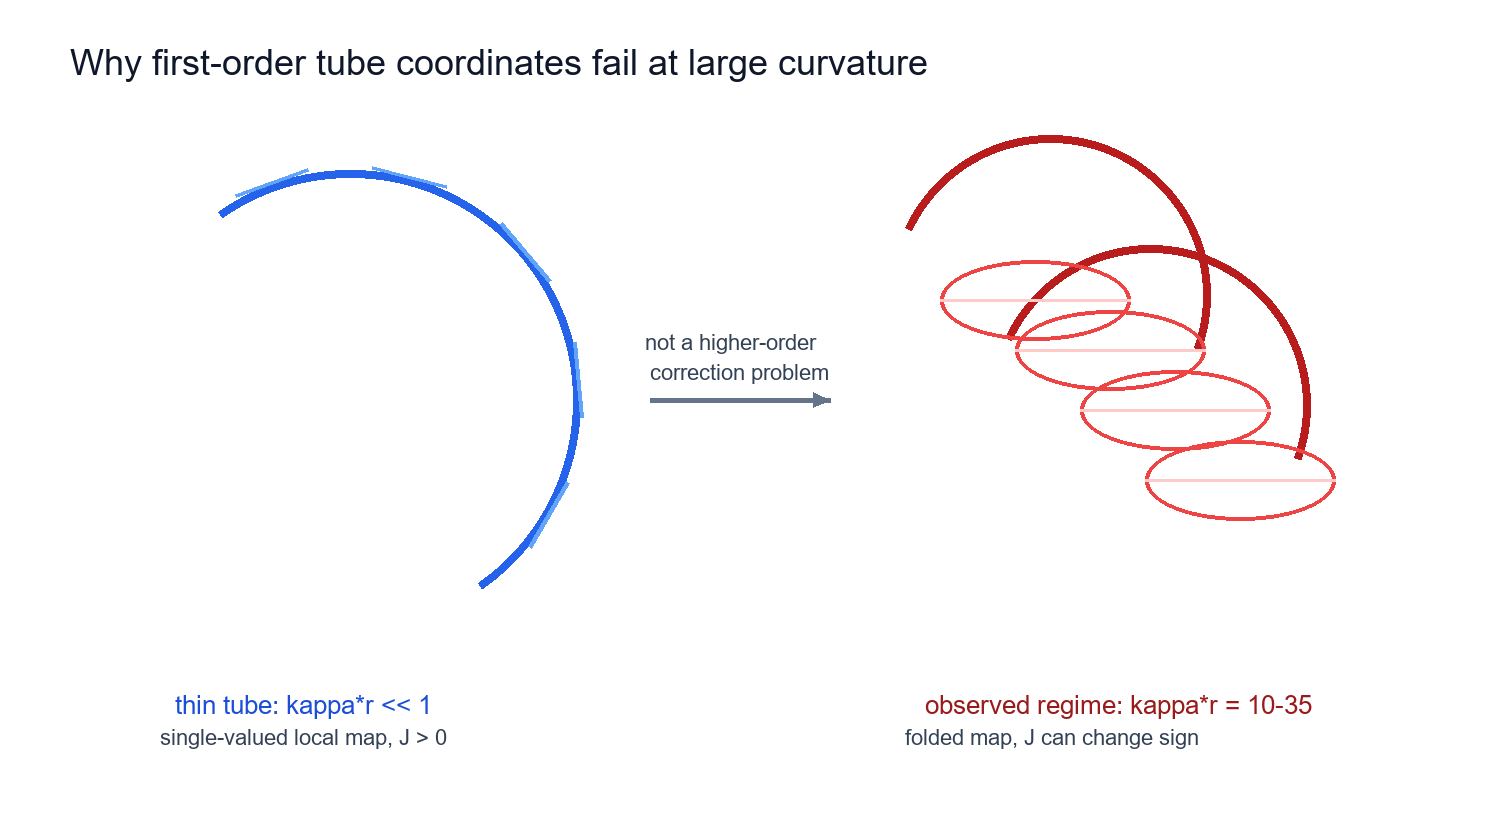
\includegraphics[width=0.93\linewidth]{mv_ep_curvature_failure.png}
  \caption{一阶曲管坐标只在 $\kappa r\ll1$ 时有效。当前结果处于 $\kappa r\gg1$ 区间，
  $J$ 可变号，说明局地坐标贴图发生折叠，不能再把 Jacobian/Christoffel 项作为闭合 forcing。}
\end{figure}

\section{从细涡管到 coherent 材料体}

大曲率情形下，涡旋本体应由 coherent PV anomaly 或流函数核定义为三维材料体：
\[
  \VV(t)=
  \left\{
  \bx:\ q_c(\bx,t)\in Q_c,\quad
  \bx\ \text{属于同一 coherent 连通核}
  \right\}.
\]
边界为
\[
  \SSS(t)=\partial\VV(t),
\]
并随 coherent 结构移动。若边界是严格材料边界，则
\[
  \left(\bu-\bU_{\SSS}\right)\cdot\bn=0.
\]
若实际识别边界来自离散阈值或生命周期合成，则该条件应写成诊断误差项，而不能被默认消去。

全局 PV 加权质心定义为
\[
  \bR_c(t)
  =
  \frac{\int_{\VV(t)}\bx\,q_c\,\dd V}
       {\int_{\VV(t)}q_c\,\dd V}.
\]
也可以在每个深度层、等密度面或等 PV 壳上定义局地质心，并把这些局地质心连成
axis skeleton。这里的轴线只是诊断骨架，用来描述 tilt、bend 和 drift；它不再是坐标系统的根基。

\begin{figure}[H]
  \centering
  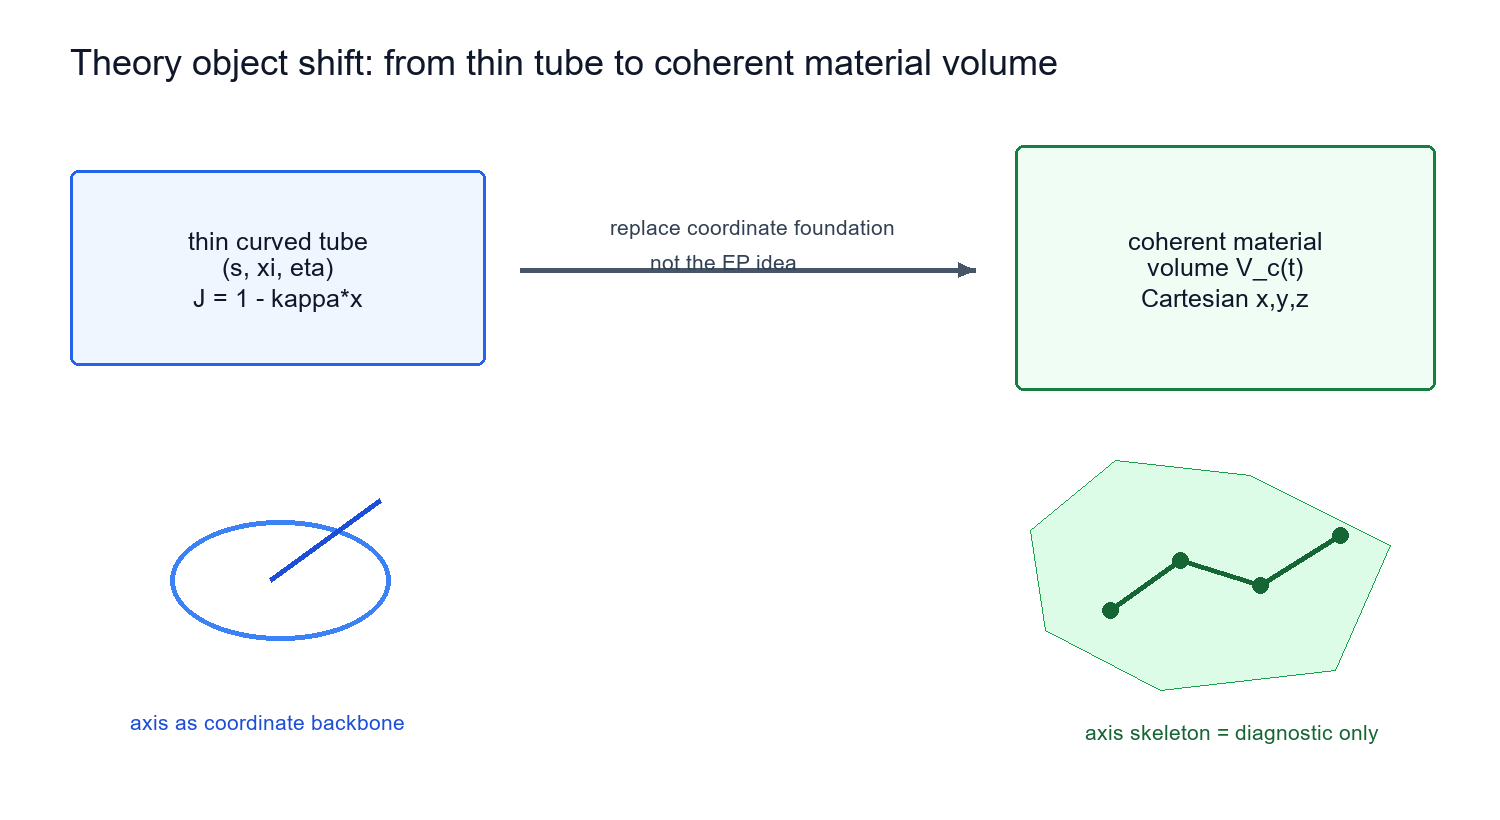
\includegraphics[width=0.93\linewidth]{mv_ep_object_shift.png}
  \caption{理论对象从 thin tube 变为 coherent material volume。轴线仍可由分层 PV 质心构造，
  但它只用于诊断形态演化，不承担全局坐标映射。}
\end{figure}

\section{材料体平均与扰动}

在材料体内定义体平均
\[
  |\VV|=\int_{\VV(t)}\dd V,\qquad
  \meanV{\phi}
  =
  \frac{1}{|\VV|}\int_{\VV(t)}\phi\,\dd V.
\]
扰动定义为
\[
  \fluc{\phi}=\phi-\meanV{\phi},
  \qquad
  \meanV{\fluc{\phi}}=0.
\]
若需要保留垂向结构，可使用分层材料体平均
\[
  \left\langle \phi\right\rangle_{V,z}
  =
  \frac{1}{A_c(z,t)}
  \int_{\VV(t)\cap z}\phi\,\dd A,
\]
其中 $A_c(z,t)$ 是 coherent 截面面积。注意这不是细管坐标截面平均；它只是 Cartesian 空间中
对实际 coherent 截面的面积积分。

\section{Cartesian 通量张量}

取 QG/Boussinesq 框架，热变量统一写成浮力
\[
  b=-g\rho'/\rho_0.
\]
在全局 Cartesian 坐标 $x_i=(x,y,z)$ 中定义三类基本通量：
\[
  R_{ij}
  =
  \meanV{\fluc{u_i}\fluc{u_j}},
  \qquad
  B_i
  =
  \meanV{\fluc{u_i}\fluc{b}},
  \qquad
  P_i
  =
  \meanV{\fluc{u_i}\fluc{q}}.
\]
$R_{ij}$ 是扰动动量通量，$B_i$ 是扰动浮力通量，$P_i$ 是 PV 通量。传统 E-P flux 的价值在于
它不把这些量分开解释，而是利用平衡关系把动量通量和热/浮力通量组合成同一个平均流强迫。

大曲率材料体版本的局地强迫写成
\[
  \boxed{
  \GG_i
  =
  -\p_j\left(\rho_0 R_{ij}\right)
  +
  \p_j\left(\rho_0\,\TT_{ij}[B_j]\right)
  }
\]
其中 $\TT_{ij}$ 是由 QG 热成风关系和 PV 反演确定的映射算子。它的作用是把浮力通量折算为
对第 $i$ 个动量分量的平衡强迫贡献。这个式子是大曲率下对传统
\[
  \rho_0^{-1}\nabla\cdot\boldsymbol F
\]
的替代：不再需要曲线坐标 Jacobian，也不需要 Christoffel 一阶闭合。

\begin{figure}[H]
  \centering
  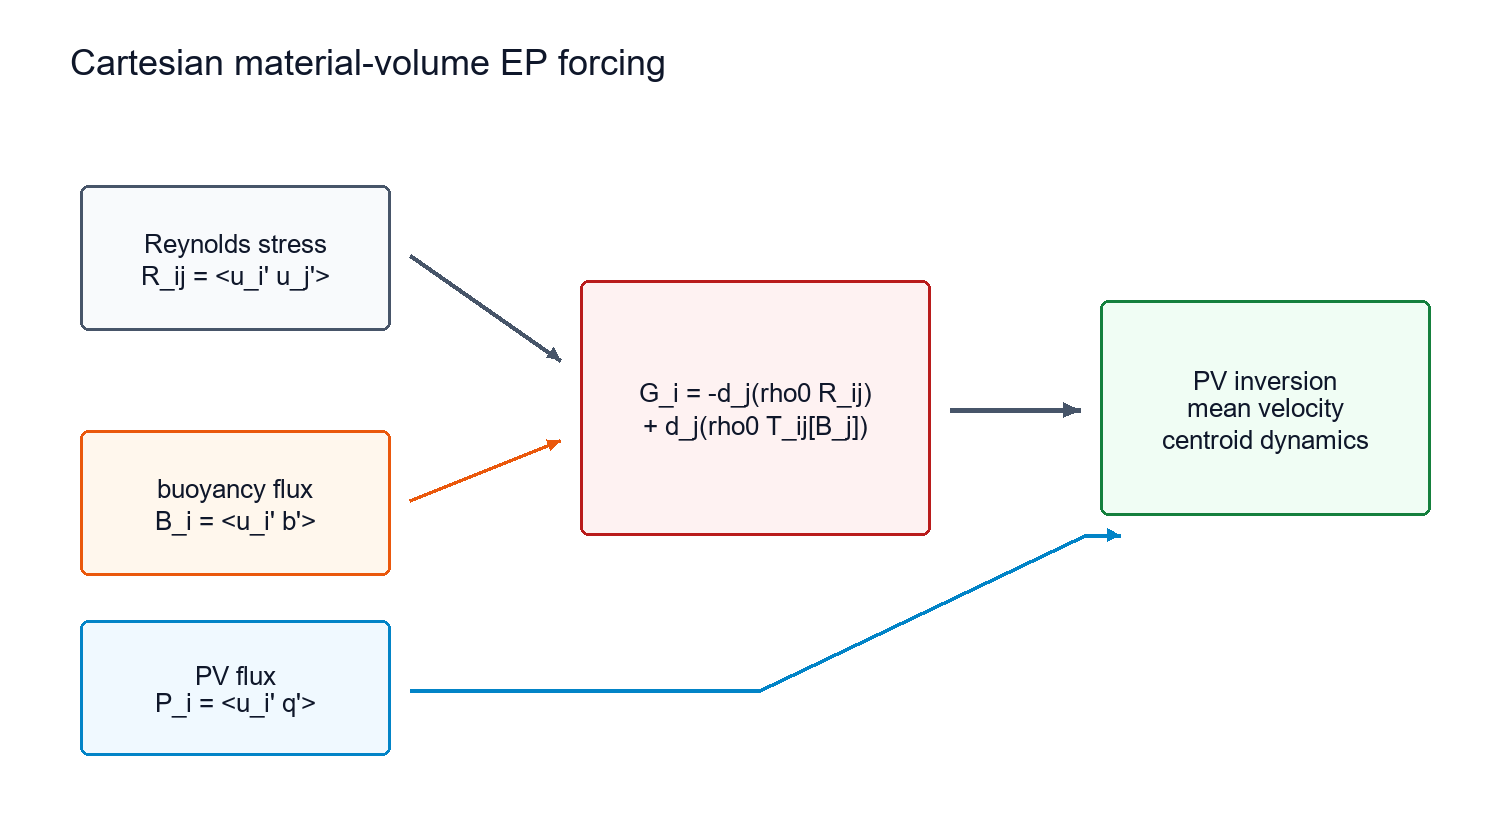
\includegraphics[width=0.93\linewidth]{mv_ep_tensor_forcing.png}
  \caption{Cartesian 材料体 EP 强迫。扰动动量通量、浮力通量和 PV 通量在全局坐标中定义，
  通过张量散度与 PV 反演共同控制 coherent 体的平均动力。}
\end{figure}

\section{边界积分形式}

对任意 coherent 材料体，体积分形式和边界积分形式通过 Gauss 定理相连：
\[
  \int_{\VV}\GG_i\,\dd V
  =
  -\int_{\SSS}\rho_0 R_{ij}n_j\,\dd S
  +
  \int_{\SSS}\rho_0\,\TT_{ij}[B_j]\,n_j\,\dd S.
\]
这个式子是大曲率版本最稳健的表达。它只依赖真实三维边界法向 $\bn$ 和全局 Cartesian 张量，
不要求边界能被一个沿轴线单射的 $(s,\xi,\eta)$ 坐标覆盖。

若边界不是严格材料面，则还需保留穿透项
\[
  \int_{\SSS} \phi\left(\bu-\bU_{\SSS}\right)\cdot\bn\,\dd S,
\]
它代表阈值漂移、混合、非保守 PV 源或识别误差。该项不应被吸收到 E-P flux 中，否则会混淆
波-平均流相互作用与边界定义误差。

\section{PV 质心速度与轴线诊断}

令
\[
  M_q(t)=\int_{\VV}q_c\,\dd V.
\]
对 PV 质心求材料导数，可得到诊断形式
\[
  \bV_c
  =
  \frac{1}{M_q}
  \int_{\VV}\bu\,q_c\,\dd V
  +
  \frac{1}{M_q}
  \int_{\VV}\left(\bx-\bR_c\right)S_q\,\dd V
  +
  \bV_{\partial V},
\]
其中 $S_q$ 是非保守 PV 源，$\bV_{\partial V}$ 是非材料边界、离散识别和合成过程带来的边界项。
将速度和 PV 分解为平均与扰动，可写成
\[
  V_{c,i}
  =
  \meanV{u_i}
  +
  \frac{|\VV|}{M_q}\meanV{\fluc{u_i}\fluc{q_c}}
  +
  V_{\mathrm{src},i}
  +
  V_{\partial V,i}.
\]
因此，PV 通量协方差仍是轴线漂移的核心量；材料体 EP 强迫 $\GG_i$ 则通过 QG/PV 反演改变
速度场和 PV 通量结构。

若用分层 PV 质心构造 axis skeleton，令弧长参数为 $s$，切向量为
\[
  \bt=\p_s\bR_c(s,t),\qquad |\bt|=1.
\]
则形态演化仍满足
\[
  \D_t\bt
  =
  \p_s\bV_c
  -
  \left(\bt\cdot\p_s\bV_c\right)\bt
  =
  \PP\,\p_s\bV_c,
  \qquad
  \PP=\boldsymbol I-\bt\bt.
\]
这条式子在大曲率下仍可用，因为它是空间曲线的运动学恒等式，不依赖小曲率坐标展开。

\begin{figure}[H]
  \centering
  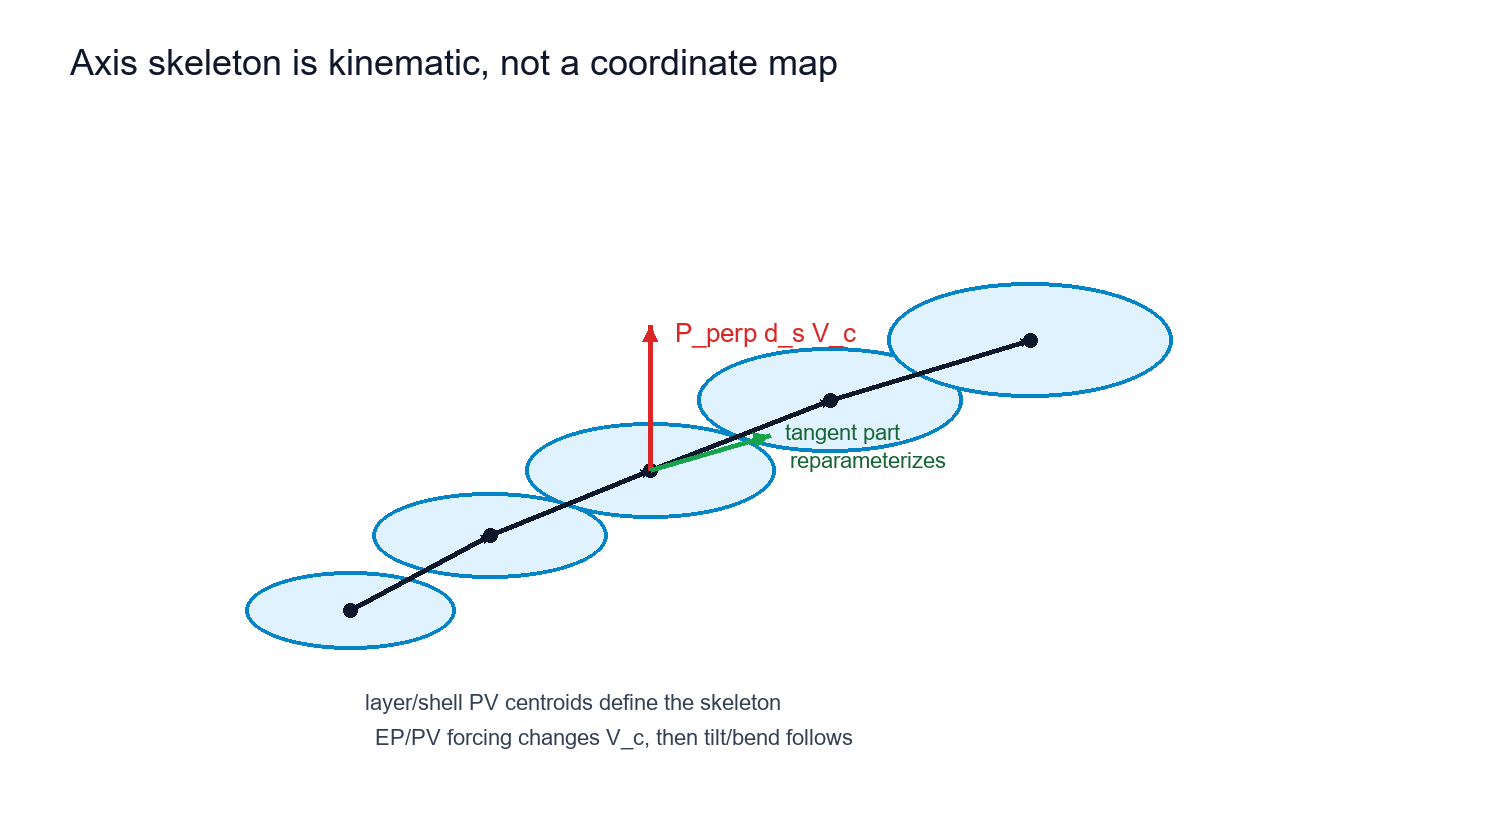
\includegraphics[width=0.90\linewidth]{mv_ep_axis_skeleton.png}
  \caption{轴线作为诊断骨架。EP/PV 通量先改变材料体内的速度和 PV 质心速度，
  再通过 $\PP\,\partial_s\bV_c$ 改变 tilt 和 bend。}
\end{figure}

\section{与小曲率 curved-tube 的关系}

当 coherent 体退化为细直管或弱弯曲管，并满足
\[
  \kappa r\ll1,\qquad J=1-\kappa_\alpha x^\alpha>0,
\]
材料体边界可由单一管坐标覆盖。此时 Cartesian 体积分可投影到局地截面，
张量散度可近似为带 Jacobian 的曲管散度，进一步在直轴、圆截面和统计轴对称极限下回到传统
TEM/E-P flux 结构。

反过来，当 $\kappa r\ge 1$、$J\le0$ 或 metric valid fraction 很低时，旧曲管文档中的
一阶曲管表达只能保留为尺度审计。可以报告曲率上界、Jacobian 最小值和 metric valid fraction，
但不能把一阶 Jacobian 修正或一阶 Christoffel 近似作为物理闭合结论。

\section{后续诊断路线}

第一版数值诊断应按以下顺序推进：
\begin{enumerate}[label=\arabic*.]
  \item 用 coherent PV anomaly 或流函数核识别三维连通材料体 $\VV(t)$。
  \item 在 Cartesian 网格上计算体平均、分层平均、$R_{ij}$、$B_i$ 和 $P_i$。
  \item 对真实三维边界 $\SSS$ 计算法向 $\bn$、面积元 $\dd S$ 和边界通量。
  \item 使用 QG/Boussinesq PV 反演确定 $\TT_{ij}$ 或至少给出可审计的离散近似。
  \item 以 $\GG_i$ 与 PV 通量散度为主解释量，继续保留 tilted EP 作为可比较的低阶诊断。
  \item 用 per-track accumulator 做 bootstrap/jackknife，避免从最终均值代表涡伪造置信区间。
\end{enumerate}

\section{一句话总结}

大曲率中尺度涡不能再被当作细弯管来展开；应把它看作 coherent PV 材料体，在全局 Cartesian
坐标中计算扰动动量通量、浮力通量、PV 通量及其边界积分。最终控制 coherent tilt 和弯曲的仍是
\[
  \PP\,\p_s\bV_c,
\]
但 $\bV_c$ 的来源应由材料体 PV 质心动力、Cartesian EP 张量强迫和真实边界项共同给出。

\end{document}
